\section{What the training objective does and does not require}
\label{sec:theory}

We state two simple facts that frame the experiments. Neither is deep; both are routinely ignored
when probing results and OOD failures of world models are interpreted.

\paragraph{Setting.} A world situation $\omega$ (state plus parameters, e.g.\ gravity $g$)
generates context observations $c$ and future observations $Y = F(\omega) \in \mathbb{R}^m$
(e.g.\ object positions over a horizon). A world model maps $c$ to a belief state $h = h(c)$
and predicts $\hat Y = P(h)$. Let $q(\omega)$ be a scalar quantity (energy, $g$, \dots).

\begin{proposition}[Competence implies decodability]
\label{prop:decode}
Suppose futures separate $q$ with modulus $\kappa > 0$:
$\|F(\omega) - F(\omega')\| \ge \kappa\, |q(\omega) - q(\omega')|$ for all $\omega, \omega'$
in the support, and the model is uniformly $\varepsilon$-accurate:
$\|P(h(c(\omega))) - F(\omega)\| \le \varepsilon$. Then there is a decoder $D$ with
$|D(h) - q(\omega)| \le 2\varepsilon/\kappa$ on the support.
\end{proposition}
\begin{proof}
Given $h$, choose any $\omega^\star$ with $\|F(\omega^\star) - P(h)\| \le \varepsilon$
(one exists: the true $\omega$) and set $D(h) = q(\omega^\star)$. Then
$\kappa |q(\omega^\star) - q(\omega)| \le \|F(\omega^\star) - F(\omega)\|
\le \|F(\omega^\star) - P(h)\| + \|P(h) - F(\omega)\| \le 2\varepsilon$.
\end{proof}
Gravity is separated by free-flight futures with
$\kappa \propto \|(t^2/2)_{t}\|$, and energy is separated by the apex heights it implies. So any
accurate predictor must carry $g$ and $E$ in its state, in some (possibly nonlinear) code. A
successful probe is therefore implied by low loss alone. It shows that the model predicts well,
not that it ``knows physics'' in any further sense. This is why we do not treat decodability
(E1) as the main evidence and turn to interventions.

\begin{proposition}[Bayes-optimal predictors clamp out-of-range parameters]
\label{prop:clamp}
Consider free flight, $y(t) = y_0 + v_0 t - \tfrac12 g t^2$, with a training prior on $g$
supported on $[a, b]$. Let $f^\star(c, t) = \mathbb{E}[y(t)\mid c]$ be the squared-loss optimal
prediction, and define its implied gravity as $-2\times$ the $t^2$-coefficient of
$t \mapsto f^\star(c, t)$. Then:
\begin{enumerate}
\item[(i)] the implied gravity equals the posterior mean $\mathbb{E}[g\mid c]$, which lies in
$[a,b]$ for every context $c$ at which the posterior is defined;
\item[(ii)] if the context positions carry i.i.d.\ Gaussian noise of variance $\sigma^2 > 0$ and
the true gravity is $g^\star > b$, the implied gravity converges to $b$ as the number of context
frames grows (symmetrically, to $a$ if $g^\star < a$);
\item[(iii)] without observation noise, contexts generated by $g^\star \notin [a,b]$ have
probability zero under training, so the expected loss does not depend on the predictor's output
there: any extrapolation, lawful or not, is equally optimal.
\end{enumerate}
\end{proposition}
\begin{proof}
(i) By linearity of conditional expectation,
$f^\star(c,t) = \mathbb{E}[y_0\mid c] + \mathbb{E}[v_0\mid c]\,t - \tfrac12\mathbb{E}[g\mid c]\,t^2$,
a quadratic in $t$ with implied gravity $\mathbb{E}[g\mid c]$. Since the posterior is supported
on the prior's support $[a,b]$, its mean lies in $[a,b]$.
(ii) With flat priors on $(y_0, v_0)$, the marginal likelihood of $g$ given $n$ noisy positions is
Gaussian, $\mathcal{N}(\hat g_n; g, s_n^2)$, where $\hat g_n$ is the least-squares curvature
estimate and $s_n \to 0$. The posterior is the normal $\mathcal{N}(\hat g_n, s_n^2)$ truncated to
$[a,b]$, whose mean is $\hat g_n - s_n \frac{\phi(\beta_n)-\phi(\alpha_n)}{\Phi(\beta_n)-\Phi(\alpha_n)}$
with $\alpha_n = (a - \hat g_n)/s_n$ and $\beta_n = (b-\hat g_n)/s_n$. As $\hat g_n \to g^\star > b$
and $s_n \to 0$, $\beta_n \to -\infty$ and the truncated mean converges to $b$.
(iii) The risk is an integral against the training distribution of contexts. A set of contexts
of measure zero does not change it.
\end{proof}

\begin{figure*}[t]
\centering
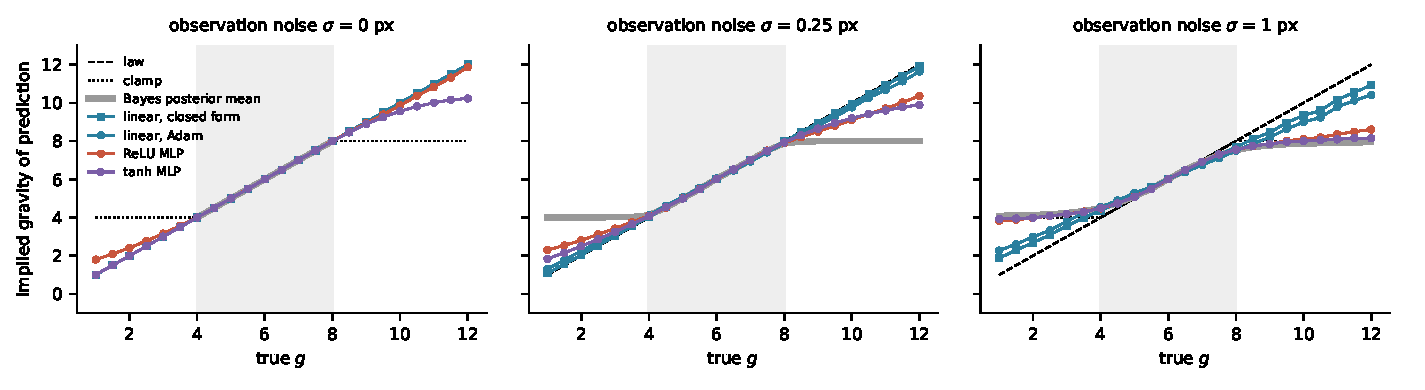
\includegraphics[width=\textwidth]{fig_toy.pdf}
\caption{Proposition~\ref{prop:clamp} in the simplest setting: 1D free fall, ten noisy context heights,
twenty future heights, squared loss, $g\sim\mathcal U[4,8]$ at training. The grey curve is the exact
posterior mean. A linear predictor (for which the law is linear in the data) extrapolates the law
when there is no noise, because then the loss does not constrain out-of-range contexts and the
least-norm solution happens to be the law; with noise its implied gravity follows the posterior
mean. ReLU and tanh MLPs trained on the same data clamp even without noise. Mean of 3 seeds.}
\label{fig:toy}
\end{figure*}

\paragraph{Consequences for experiments.} Proposition~\ref{prop:clamp} gives a reference curve
for OOD gravity. Figure~\ref{fig:toy} shows the proposition at work in a toy setting where
everything is exact; the caption is written before the toy results and may need revision.
% FINALIZE: rewrite the caption from results/v2/toy_bayes.json. The \emph{law} is $g_{\rm eff} = g^\star$, and the \emph{Bayes-optimal}
response is approximately $\mathrm{clamp}(g^\star, a, b)$, softened by noise
(Fig.~\ref{fig:locus}a shows the exact truncated-normal curve for our contexts). A model that
snaps back is therefore doing what its loss asks. A model that extrapolates does so because of an
inductive bias that the loss does not specify. Two further points matter for interpreting
interventions. First, the Bayes predictor can be built so that its belief state stores the
\emph{unclamped} sufficient statistic $\hat g_n$ and applies the clamp only when it predicts.
Clamping can therefore live in ``inference'' or in ``execution'', and the theory does not say
which. That is an empirical question, and Section~\ref{sec:locus} answers it with probes and
steering. Second, (iii) means that what happens out of range is decided by the architecture's
extrapolation behaviour. ReLU and GRU networks are known to extrapolate roughly linearly along
some directions \citep{xu2021extrapolate}, so partial extrapolation is a priori plausible.
